%% For double-blind review submission, w/o CCS and ACM Reference (max submission space)
\documentclass[sigplan,10pt,review]{acmart} %anonymous
\settopmatter{printfolios=true,printccs=false,printacmref=false}
%% For double-blind review submission, w/ CCS and ACM Reference
%\documentclass[sigplan,review,anonymous]{acmart}\settopmatter{printfolios=true}
%% For single-blind review submission, w/o CCS and ACM Reference (max submission space)
%\documentclass[sigplan,review]{acmart}\settopmatter{printfolios=true,printccs=false,printacmref=false}
%% For single-blind review submission, w/ CCS and ACM Reference
%\documentclass[sigplan,review]{acmart}\settopmatter{printfolios=true}
%% For final camera-ready submission, w/ required CCS and ACM Reference
%\documentclass[sigplan]{acmart}\settopmatter{}


%% Conference information
%% Supplied to authors by publisher for camera-ready submission;
%% use defaults for review submission.
\acmConference[PL'18]{ACM SIGPLAN Conference on Programming Languages}{January 01--03, 2018}{New York, NY, USA}
\acmYear{2018}
\acmISBN{} % \acmISBN{978-x-xxxx-xxxx-x/YY/MM}
\acmDOI{} % \acmDOI{10.1145/nnnnnnn.nnnnnnn}
\startPage{1}

%% Copyright information
%% Supplied to authors (based on authors' rights management selection;
%% see authors.acm.org) by publisher for camera-ready submission;
%% use 'none' for review submission.
\setcopyright{none}
%\setcopyright{acmcopyright}
%\setcopyright{acmlicensed}
%\setcopyright{rightsretained}
%\copyrightyear{2018}           %% If different from \acmYear

%% Bibliography style
\bibliographystyle{ACM-Reference-Format}
%% Citation style
%\citestyle{acmauthoryear}  %% For author/year citations
%\citestyle{acmnumeric}     %% For numeric citations
%\setcitestyle{nosort}      %% With 'acmnumeric', to disable automatic
                            %% sorting of references within a single citation;
                            %% e.g., \cite{Smith99,Carpenter05,Baker12}
                            %% rendered as [14,5,2] rather than [2,5,14].
%\setcitesyle{nocompress}   %% With 'acmnumeric', to disable automatic
                            %% compression of sequential references within a
                            %% single citation;
                            %% e.g., \cite{Baker12,Baker14,Baker16}
                            %% rendered as [2,3,4] rather than [2-4].


%%%%%%%%%%%%%%%%%%%%%%%%%%%%%%%%%%%%%%%%%%%%%%%%%%%%%%%%%%%%%%%%%%%%%%
%% Note: Authors migrating a paper from traditional SIGPLAN
%% proceedings format to PACMPL format must update the
%% '\documentclass' and topmatter commands above; see
%% 'acmart-pacmpl-template.tex'.
%%%%%%%%%%%%%%%%%%%%%%%%%%%%%%%%%%%%%%%%%%%%%%%%%%%%%%%%%%%%%%%%%%%%%%


%% Some recommended packages.
\usepackage{booktabs}   %% For formal tables:
                        %% http://ctan.org/pkg/booktabs
\usepackage{subcaption} %% For complex figures with subfigures/subcaptions
                        %% http://ctan.org/pkg/subcaption'
%%%%%%%%%%%%%%%%%%%%%%%%%%%%%%%%
\usepackage{graphicx}
\usepackage{algpseudocode}
\usepackage{algorithm}
\usepackage{algorithmicx}
\usepackage{verbatim}
\usepackage{mathtools}
\usepackage{multirow}
\usepackage{colortbl}
\usepackage{balance}
\usepackage{hyperref}
\usepackage{subcaption}


\usepackage{dirtree}

\usepackage{natbib}
\usepackage{amssymb}

\usepackage{tikz}
\usetikzlibrary{fit,automata,positioning}
\usetikzlibrary{decorations.pathmorphing}
\tikzset{snake it/.style={decorate, decoration=snake}}
\usepackage{kbordermatrix} % include package @ document preamble
%%%%%%%%%%%%%%%%%%%%%%%%%%%%%%%%%%%%%
\newcommand\mc{\multicolumn{1}{c}{\cellcolor{lightgray}\textbf{1}}}
\newcommand{\term}[1]{\emph{#1}}
%%%%%%%%%%%%%%%%%%%%%%%%%%%%%%%%%%%%%%%

\begin{document}

%% Title information
\title[Linear Algebra Based CFL-reachability]{?One Algorithm to Evaluate Them All: Unified Linear Algebra Based Approach to Evaluate Both Regular and Context-Free Path Queries?}         %% [Short Title] is optional;
                                        %% when present, will be used in
                                        %% header instead of Full Title.
\titlenote{The research was supported by the Russian Science Foundation, grant number: 18-11-00100}             %% \titlenote is optional;
                                        %% can be repeated if necessary;
                                        %% contents suppressed with 'anonymous'
%\subtitle{Subtitle}                     %% \subtitle is optional
%\subtitlenote{with subtitle note}       %% \subtitlenote is optional;
                                        %% can be repeated if necessary;
                                        %% contents suppressed with 'anonymous'


%% Author information
%% Contents and number of authors suppressed with 'anonymous'.
%% Each author should be introduced by \author, followed by
%% \authornote (optional), \orcid (optional), \affiliation, and
%% \email.
%% An author may have multiple affiliations and/or emails; repeat the
%% appropriate command.
%% Many elements are not rendered, but should be provided for metadata
%% extraction tools.


%% Author with two affiliations and emails.
\author{Ekaterina Shemetova}
%\authornote{with author2 note}          %% \authornote is optional;
                                        %% can be repeated if necessary
\orcid{nnnn-nnnn-nnnn-nnnn}             %% \orcid is optional
\affiliation{
 % \position{Position2a}
 % \department{Department2a}             %% \department is recommended
  \institution{Saint Petersburg State University}           %% \institution is required
  \streetaddress{7/9 Universitetskaya nab.}
  %\city{St. Petersburg}
  %\state{State2a}
  %\postcode{Post-Code2a}
  %\country{Russia}                   %% \country is recommended
}

\affiliation{
 % \position{Position2a}
 % \department{Department2a}             %% \department is recommended
  \institution{Saint Petersburg Academic University}           %% \institution is required
  \streetaddress{8/3 Khlopin St.}
 % \city{St. Petersburg}
  %\state{State2a}
  %\postcode{Post-Code2a}
%  \country{Russia}                   %% \country is recommended
}
\affiliation{
 % \position{Position2a}
 % \department{Department2a}             %% \department is recommended
  \institution{JetBrains Research}           %% \institution is required
  \streetaddress{Primorskiy prospekt 68-70, Building 1}
  \city{St. Petersburg}
  %\state{State2a}
  %\postcode{Post-Code2a}
  \country{Russia}                   %% \country is recommended
}
\email{katyacyfra@gmail.com}         %% \email is recommended

%%%%%%%%%%%%%%%%%%%%%%%%%%%%%%%%%%%%%%%%%%%%%%%%%%%
\author{Rustam Azimov}
%\authornote{with author2 note}          %% \authornote is optional;
                                        %% can be repeated if necessary
\orcid{nnnn-nnnn-nnnn-nnnn}             %% \orcid is optional
\affiliation{
 % \position{Position2a}
 % \department{Department2a}             %% \department is recommended
  \institution{Saint Petersburg State University}           %% \institution is required
  \streetaddress{7/9 Universitetskaya nab.}
  %\city{St. Petersburg}
  %\state{State2a}
  %\postcode{Post-Code2a}
  %\country{Russia}                   %% \country is recommended
}
\affiliation{
 % \position{Position2a}
 % \department{Department2a}             %% \department is recommended
  \institution{JetBrains Research}           %% \institution is required
  \streetaddress{Primorskiy prospekt 68-70, Building 1}
  \city{St. Petersburg}
  %\state{State2a}
  %\postcode{Post-Code2a}
  \country{Russia}                   %% \country is recommended
}
\email{rustam.azimov19021995@gmail.com}         %% \email is recommended
%%%%%%%%%%%%%%%%%%%%%%%%%%%%%%%%%%%%%%%%%%%%%%%%%%%
\author{ Egor Orachev }
%\authornote{with author2 note}          %% \authornote is optional;
                                        %% can be repeated if necessary
\orcid{nnnn-nnnn-nnnn-nnnn}             %% \orcid is optional
\affiliation{
 % \position{Position2a}
 % \department{Department2a}             %% \department is recommended
  \institution{Saint Petersburg State University}           %% \institution is required
  \streetaddress{7/9 Universitetskaya nab.}
  %\city{St. Petersburg}
  %\state{State2a}
  %\postcode{Post-Code2a}
  %\country{Russia}                   %% \country is recommended
}
\affiliation{
 % \position{Position2a}
 % \department{Department2a}             %% \department is recommended
  \institution{JetBrains Research}           %% \institution is required
  \streetaddress{Primorskiy prospekt 68-70, Building 1}
  \city{St. Petersburg}
  %\state{State2a}
  %\postcode{Post-Code2a}
  \country{Russia}                   %% \country is recommended
}
\email{egor.orachev@gmail.com}         %% \email is recommended
%%%%%%%%%%%%%%%%%%%%%%%%%%%%%%%%%%%%%%%%%%%%%%%%%%%
\author{Ilya Epelbaum}
%\authornote{with author2 note}          %% \authornote is optional;
                                        %% can be repeated if necessary
\orcid{nnnn-nnnn-nnnn-nnnn}             %% \orcid is optional
\affiliation{
 % \position{Position2a}
 % \department{Department2a}             %% \department is recommended
  \institution{Saint Petersburg State University}           %% \institution is required
  \streetaddress{7/9 Universitetskaya nab.}
  %\city{St. Petersburg}
  %\state{State2a}
  %\postcode{Post-Code2a}
  %\country{Russia}                   %% \country is recommended
}
\affiliation{
 % \position{Position2a}
 % \department{Department2a}             %% \department is recommended
  \institution{JetBrains Research}           %% \institution is required
  \streetaddress{Primorskiy prospekt 68-70, Building 1}
  \city{St. Petersburg}
  %\state{State2a}
  %\postcode{Post-Code2a}
  \country{Russia}                   %% \country is recommended
}
\email{iliyepelbaun@gmail.com}         %% \email is recommended
%%%%%%%%%%%%%%%%%%%%%%%%%%%%%%%%%%%%%%%%%%%%%%%%%%%
\author{Alexandra Olemskaya}
%\authornote{with author2 note}          %% \authornote is optional;
                                        %% can be repeated if necessary
\orcid{nnnn-nnnn-nnnn-nnnn}             %% \orcid is optional
\affiliation{
 % \position{Position2a}
 % \department{Department2a}             %% \department is recommended
  \institution{National Research University Higher School of Economics }           %% \institution is required
 % \streetaddress{}
  \city{St. Petersburg}
  %\state{State2a}
  %\postcode{Post-Code2a}
  \country{Russia}                   %% \country is recommended
}
\email{alexandra.olemskaya@gmail.com }         %% \email is recommended
%%%%%%%%%%%%%%%%%%%%%%%%%%%%%%%%%%%%%%%%%%%%%%%%%%%
\author{Semyon Grigorev}
%\authornote{with author2 note}          %% \authornote is optional;
                                        %% can be repeated if necessary
\orcid{nnnn-nnnn-nnnn-nnnn}             %% \orcid is optional
\affiliation{
 % \position{Position2a}
 % \department{Department2a}             %% \department is recommended
  \institution{Saint Petersburg State University}           %% \institution is required
  \streetaddress{7/9 Universitetskaya nab.}
  %\city{St. Petersburg}
  %\state{State2a}
  %\postcode{Post-Code2a}
  %\country{Russia}                   %% \country is recommended
}
\affiliation{
 % \position{Position2a}
 % \department{Department2a}             %% \department is recommended
  \institution{JetBrains Research}           %% \institution is required
  \streetaddress{Primorskiy prospekt 68-70, Building 1}
  \city{St. Petersburg}
  %\state{State2a}
  %\postcode{Post-Code2a}
  \country{Russia}                   %% \country is recommended
}
\email{s.v.grigoriev@spbu.ru}         %% \email is recommended
\email{semyon.grigorev@jetbrains.com}         %% \email is recommended


%% Abstract
%% Note: \begin{abstract}...\end{abstract} environment must come
%% before \maketitle command
\begin{abstract}
  The Kronecker product-based algorithm for context-free path querying (CFPQ) was proposed by \cite{10.1007/978-3-030-54832-2_6}. We reduce this algorithm to operations over Boolean matrices and extend it with the mechanism to extract all paths of interest. We also prove $O(n^3/\log{n})$ time complexity of the proposed algorithm, where $n$ is a number of vertices of the input graph. Thus, we provide the alternative way to construct a slightly subcubic algorithm for CFPQ which is based on linear algebra and incremental transitive closure
  (a classic graph-theoretic problem), as opposed to the algorithm with the same complexity proposed by~\cite{10.1145/1328438.1328460}. Our evaluation shows that our algorithm is a good candidate to be the universal algorithm for both regular and context-free path querying.
\end{abstract}


%% 2012 ACM Computing Classification System (CSS) concepts
%% Generate at 'http://dl.acm.org/ccs/ccs.cfm'.
\begin{CCSXML}
<ccs2012>
<concept>
<concept_id>10011007.10011006.10011008</concept_id>
<concept_desc>Software and its engineering~General programming languages</concept_desc>
<concept_significance>500</concept_significance>
</concept>
<concept>
<concept_id>10003456.10003457.10003521.10003525</concept_id>
<concept_desc>Social and professional topics~History of programming languages</concept_desc>
<concept_significance>300</concept_significance>
</concept>
</ccs2012>
\end{CCSXML}

\ccsdesc[500]{Software and its engineering~General programming languages}
\ccsdesc[300]{Social and professional topics~History of programming languages}
%% End of generated code


%% Keywords
%% comma separated list
\keywords{CFL-reachability, Static Analysis, Linear Algebra}  %% \keywords are mandatory in final camera-ready submission


%% \maketitle
%% Note: \maketitle command must come after title commands, author
%% commands, abstract environment, Computing Classification System
%% environment and commands, and keywords command.
\maketitle


\section{Introduction}

Scalable high-performance graph analysis is an actual challenge.
There is a big number of ways to attack this challenge~\cite{Coimbra2021} and the first promising idea is to utilize general-purpose graphic processing units (GPGPU-s).
Such existing solutions, as CuSha~\cite{10.1145/2600212.2600227} and Gunrock~\cite{7967137} show that utilization of GPUs can improve the performance of graph analysis, moreover it is shown that solutions may be scaled to multi-GPU systems.
But low flexibility and high complexity of API are problems of these solutions.

The second promising thing which provides a user-friendly API for high-performance graph analysis algorithms creation is a GraphBLAS API~\cite{7761646} which provides linear algebra based building blocks to create graph analysis algorithms.
The idea of GraphBLAS is based on is a well-known fact that linear algebra operations can be efficiently implemented on parallel hardware.
Along with this, a graph can be natively represented using matrices: adjacency matrix, incidence matrix, etc.
While reference CPU-based implementation of GraphBLAS, SuiteSparse:GraphBLAS~\cite{10.1145/3322125}, demonstrates good performance in real-world tasks, GPU-based implementation is challenging.

One of the challenges in this way is that real data are often sparse, thus underlying matrices and vectors are also sparse, and, as a result, classical dense data structures and respective algorithms are inefficient. 
So, it is necessary to use advanced data structures and procedures to implement sparse linear algebra, but the efficient implementation of them on GPU is hard due to the irregularity of workload and data access patterns.
Though such well-known libraries as cuSparse show that sparse linear algebra operations can be efficiently implemented for GPGPU-s, it is not so trivial to implement GraphBLAS on GPGPU. 
First of all, it requires \textit{generic} sparse linear algebra, thus it is impossible just to reuse existing libraries which are almost all specified for operations over floats.
The second problem is specific optimizations, such as maskings fusion, which can not be natively implemented on top of existing kernels.
Nevertheless, there is a number of implementations of GraphBLAS on GPGPU, such as GraphBLAST:~\cite{yang2019graphblast}, GBTL~\cite{7529957}, which show that GPGPUs utilization can improve the performance of GraphBLAS-based graph analysis solutions.
But these solutions are not portable because they are based on Nvidia Cuda stack.
Moreover, the scalability problem is not solved: all these solutions support only single-GPU, not multi-GPU computations.

To provide portable GPU implementation of GraphBLAS API we developed a \textit{SPLA} library (sources are published on GitHub: \url{https://github.com/JetBrains-Research/spla}).
This library utilizes OpenCL for GPGPU computing to be portable across devices of different vendors.
Moreover, it is initially designed to utilize multiple GPGPUs to be scalable.
To sum up, the contribution of this work is the following.
\begin{itemize}
    \item Design of portable GPU GraphBLAS implementation proposed. The design involves the utilization of multipole GPUS. Additionally, the proposed design is aimed to simplify library tuning and wrappers for different high-level platforms and languages creation. 
    \item Subset of GraphBLAS API, including such operations as masking, matrix-matrix multiplication, matrix-matrix e-wise addition, is implemented. The current implementation is limited by COO and CSR matrix representation format and uses basic algorithms for some operations, but work in progress and more data formats will be supported and advanced algorithms will be implemented in the future.
    \item Preliminary evaluation on such algorithms as breadth-first search (BFS) and triangles counting (TC), and real-world graphs shows portability across different vendors and promising performance: for some problems Spla is comparable with GraphBLAST. Surprisingly, for some problems, the proposed solution on embedded Intel graphic card shows better performance than SuiteSparse:GraphBLAS on the same CPU. At the same time, the evaluation shows that further optimization is required.
\end{itemize} 
\section{Preliminaries}

We introduce !!!!

\subsection{Context-Free Path Querying}

Graph, grammar, etc.

Let $i\pi j$ denote a unique path between nodes $i$ and $j$ of the graph and $l(\pi)$ denotes a unique string which is obtained from the concatenation of edge labels along the path $\pi$.
For a context-free grammar $G = (\Sigma, N, P, S)$ and directed labelled graph $D = (Q, \Sigma, \delta)$, a triple $(A, i, j)$ is \textit{realizable} iff there is a path $i\pi j$ such that nonterminal $A \in N$ derives $l(\pi)$.

\subsection{Tensor-Based algorithm for CFPQ}

\begin{algorithm}[H]
\begin{algorithmic}[1]
\caption{Kronecker product context-free recognizer for graphs}
\label{alg:Kronecker}
\Function{contextFreePathQuerying}{D, G}
\EndFunction
\end{algorithmic}
\end{algorithm}

\subsection{Planar Graphs}

A planar graph $G = (V, E)$ is a graph that can be embedded in the plane.

Outer face - unbounded face in specific embedding.

Directed graph (\textit{digraph})

...

\subsection{Dynamic reachability algorithms}

We consider algorithms that solve the problem of reachability in planar directed graphs. In the \textit{dynamic reachability problem} we are given a graph $G$ subject to edge updates (insertions or deletions) and the goal is to design a data structure that would allow answering queries about the existence of a path.

We need to answer the queries of type: "Is there a directed path from $u$ to $v$ in $G$?". If vertex $u$ in all the queries is fixed we say that algorithm is \textit{single-source}. It is said to be \textit{all-pairs} if vertices $u, v$ can be any vertices of planar digraph $G$, in this case it can be also called \textit{dynamic transitive closure}.

We say that the algorithm is \textit{fully dynamic} if it supports both additions and deletions of edges. It is said to be \textit{semi dynamic} if it supports only one of these updates. If semi dynamic algorithm supports additions only it is called \textit{incremental}, if deletions only - \textit{decremental}.






\section{Context-free path querying by Kronecker product}


In this section, we introduce the algorithm for context-free path querying which is based on the Kronecker product of Boolean matrices.
The algorithm solves all-pairs CFPQ problem with all-path semantics (according to~\cite{hellingsPathQuerying}).
The algorithm works in the following two steps.
\begin{enumerate}
\item \emph{Index creation}.
 During this step, the algorithm computes an index that contains the information necessary to restore paths for the given pairs of vertices.
 This index can be used to solve the reachability problem without extracting paths.
 Note that the index is finite even when the set of paths is infinite.
\item \emph{Paths extraction}.
All paths for the given pair of vertices can be enumerated by using the index.
Since the set of paths can be infinite, all paths cannot be enumerated explicitly, thus advanced techniques such as lazy evaluation are required for the implementation.
Nevertheless, a single path can always be extracted with standard techniques.
\end{enumerate}

In the following subsections, we describe these steps, prove the correctness of the algorithm, and provide time complexity estimations.
For the first step, we start by introducing a naive algorithm.
After that, we show how to achieve cubic time complexity by using a dynamic transitive closure algorithm and shave off a logarithmic factor to achieve the best known time complexity for the CFPQ problem.
We finish by providing a step-by-step example of query evaluation with the proposed algorithm.

\subsection{Index Creation Algorithm}

The \textit{index creation} algorithm outputs the final adjacency matrix for the input graph with all pairs of vertices which are reachable through some nonterminal in the input grammar $G$, as well as the index matrix which is to be used to extract paths in the \textit{path extraction} algorithm.

The algorithm is based on the generalization of the FSM intersection for an RSM,  and the edge-labeled directed input graph.
Since the RSM is composed as a set of FSMs, it could easily be presented as an adjacency matrix for some graph over the set of labels.
As shown in the Def.~\ref{def:bool:product}, we can apply Kronecker product for Boolean matrices to \textit{intersect} the RSM and the input graph to some extent.
But the RSM contains nonterminal symbols with the additional logic of \textit{recursive calls}, which requires a \textit{transitive closure} step to extract such symbols.

The core idea of the algorithm comes from the Kronecker product and transitive closure.
The algorithm boils down to the evaluation of the iterative Kronecker product for the adjacency matrix $\mathcal{M}_1$ of the RSM $R$ and the adjacency matrix $\mathcal{M}_2$ of the  input graph $\mathcal{G}$, followed by the transitive closure, extraction of nonterminals and updating the graph adjacency matrix $\mathcal{M}_2$.
Listing~\ref{tensor:cfpq:cubic} demonstrates the main steps of the algorithm.
\begin{algorithm}[h]
\floatname{algorithm}{Listing}
\begin{algorithmic}[1]
\footnotesize
\caption{Kronecker product based CFPQ using dynamic transitive closure}
\label{tensor:cfpq:cubic}
\Function{contextFreePathQuerying}{G, $\mathcal{G}$}
    % Input data preparation
   \State{$n \gets$ the number of nodes in $\mathcal{G}$}
    \State{$R \gets$ recursive automata for $G$}
    \State{$\mathcal{M}_1 \gets$ the set of adjacency matrices for $R$}
    \State{$\mathcal{M}_2, \mathcal{A}_2 \gets$ the sets of adjacency matrices for $\mathcal{G}$}
    %\State{$M_3 \gets$ The empty matrix}
    \State{$C_3, M_3 \gets$ the empty matrices of size $dim(\mathcal{M}_1)n \times dim(\mathcal{M}_1)n$}
    % Eps-transition handling for graph
    \For{$s \in 0..dim(\mathcal{M}_1)-1$}
        \For{$S \in \textit{getNonterminals}(R,s,s)$}
            \For{$i \in 0..dim(\mathcal{M}_2)-1$}
                \State{$M^S_2[i,i] \gets 1 $}
            \EndFor
        \EndFor
    \EndFor
    \While{$\mathcal{M}_2$ is changing}
        \State{$M_3' \gets \bigvee_{M^S \in \mathcal{M}_1 \otimes \mathcal{A}_2} M^S$}
        \Comment{Using only new edges from $\mathcal{A}_2$}
        \State{$M_3 \gets M_3 + M_3'$}
        \Comment{Updating the matrix for the Kronecker product result}
        %\State{$\mathcal{A}_2 \gets$ The empty matrix of size $n \times n$}
        \State{$\mathcal{A}_2 \gets$ The empty matrix}
        \State{$C_3' \gets$ The empty matrix of size $dim(\mathcal{M}_1)n \times dim(\mathcal{M}_1)n$}
        %\Comment{Evaluate Kroncker product}
        \For{$(i,j) \mid M_3'[i,j] \neq 0$}
            %\State{$C_3'[i,j] \gets 1$}
            \State{$C_3' \gets \textit{add}(C_3, C_3', i, j)$}
            \Comment{Updating the transitive closure}
            \State{$C_3 \gets C_3 + C_3'$}
        \EndFor
        %\State{$n \gets$ dim($M_3)$}
        %\Comment{Matrix $M_3$ size = $n \times n$}
        % Add non-terminals (possibly new)
        \For{$(i,j)\ |\ C_3'[i,j] \neq 0$}
                \State{$s, f \gets \textit{getStates}(C_3',i,j)$}
                \State{$x, y \gets \textit{getCoordinates}(C_3',i,j)$}
                \For{$S \in \textit{getNonterminals}(R,s,f)$}
                    \State{$M^S_2[x,y] \gets 1$}
                    \State{$A^S_2[x,y] \gets 1$}
                \EndFor
        \EndFor
    \EndWhile
\State \Return $\mathcal{M}_2, M_3$
\EndFunction
% \Function{add}{$C, C', i, j$}
%     \State{$C'[i,j] \gets {1}$}
%     \For{$(u,v) \mid C[u,i] = C[j,v] = 1, C[u,j] = C[u,v] = 0$}
%         \State{$C'[u,v] \gets {1}$}
%     \EndFor
%     \State \Return{$C'$}
% \EndFunction
\Function{getStates}{$C, i, j$}
    \State{$n \gets dim(\mathcal{M}_2)$}
   \Comment{$\mathcal{M}_2$ the set of adjacency matrices for $\mathcal{G}$}
    \State \Return{$\left\lfloor{i / n}\right\rfloor, \left\lfloor{j / n}\right\rfloor$}
\EndFunction
\Function{getCoordinates}{$C, i, j$}
    \State{$n \gets dim(\mathcal{M}_2)$}
    \State \Return{$i \bmod n, j \bmod n$}
\EndFunction
\end{algorithmic}
\end{algorithm}
\subsubsection{Application of Dynamic Transitive Closure}
The most time-consuming steps of the algorithm are the computations of the Kronecker product and transitive closure.
Note that the adjacency matrix $\mathcal{M}_2$ is changed incrementally i.e. elements (edges) are added to $\mathcal{M}_2$ at each iteration of the algorithm and are never deleted from it.
So it is not necessary to recompute the whole product or transitive closure if some appropriate data structure is maintained.

To compute the Kronecker product, we employ the fact that it is left-distributive.
Let $\mathcal{A}_2$ be a matrix with newly added elements and $\mathcal{B}_2$ be a matrix with all previously found elements, such that $\mathcal{M}_2 = \mathcal{A}_2 + \mathcal{B}_2$.
Then by left-distributivity of the Kronecker product we have $\mathcal{M}_1 \otimes \mathcal{M}_2 = \mathcal{M}_1 \otimes (\mathcal{A}_2 + \mathcal{B}_2) = \mathcal{M}_1\otimes \mathcal{A}_2 + \mathcal{M}_1 \otimes \mathcal{B}_2$.
Note that $\mathcal{M}_1 \otimes \mathcal{B}_2$ is known and is already in the matrix $\mathcal{M}_3$ and its transitive closure is also already in the matrix $C_3$, because it has been calculated at the previous iterations, so it is left to update some elements of $\mathcal{M}_3$ by computing $\mathcal{M}_1\otimes \mathcal{A}_2$.


The fast computation of transitive closure can be obtained by using an incremental dynamic transitive closure technique.
Let us describe the function $add$ from Listing \ref{tensor:cfpq:cubic}.
Let $C_3$ be a transitive closure matrix of the graph $G$ with $n$ vertices.
We use an approach by~\cite{IBARAKI198395} to maintain dynamic transitive closure.
The key idea of their algorithm is to recalculate reachability information only for those vertices which become reachable after insertion of a certain edge.

We have modified the algorithm to achieve a logarithmic speed-up in the following way.
For each newly inserted edge $(i, j)$ and every node $u \neq j$ of $G$ such that $C_3[u, i] = 1$ and $C_3[u, j]=0$, one needs to perform operation $C_3[u,v] = C_3[u, v] \wedge C_3[j, v]$ for every node $v$, where $1 \wedge 1 = 0 \wedge 0 = 1 \wedge 0 = 0$ and $0 \wedge 1 = 1$.
Notice that these operations are equivalent to the element-wise (Hadamard) product of two vectors of size $n$, where multiplication operation is denoted as $\wedge$. To check whether $C_3[u, i] = 1$ and $C_3[u, j]=0$ one needs to multiply two vectors: the first vector represents reachability of the given vertex $i$ from other vertices $\{u_1, u_2, ..., u_n\}$ of the graph and the second vector represents the same for the given vertex $j$. The operation $C_3[u, v] \wedge C_3[j, v]$ also can be reduced to the computation of the Hadamard product of two vectors of size $n$ for the given $u_k$. The first vector contains the information whether vertices  $\{v_1, v_2, ..., v_n\}$ of the graph are reachable from the given vertex $u_k$ and the second vector represents the same for the given vertex $j$. The element-wise product of two vectors can be calculated naively in time $O(n)$. Thus, the time complexity of the transitive closure can be reduced by speeding up the element-wise product of two vectors of size $n$.


To achieve logarithmic speed-up, we use the Four Russians' trick.
First we split each vector into $n/\log n$ parts of size $\log n$.
Then we create a table $T$ such that $T(a, b)$ = $a \wedge b$ where $a, b \ \in {\{0,1\}}^{\log n}$.
This takes time $O(n^2 \log n)$, since there are $2^{\log n} = n$ variants of Boolean vectors of size $\log n$ and hence $n^2$ possible pairs of vectors $(a, b)$ in total, and each component takes $O(\log n)$ time.
We can calculate the product of two parts of size $\log n$ in constant time using the table $T$.
There are $n/\log n$ such parts, so the element-wise product of two vectors of size $n$ can be calculated in time $O(n/\log n)$ with $O(n^2 \log n)$ preprocessing.

\begin{theorem}
    Let $\mathcal{G} =  \langle V,E,L\rangle$ be a graph and $G = \langle\Sigma, N, S, P\rangle$ be a grammar.
    Let $\mathcal{M}_{2}$ be a resulting adjacency matrix after the execution of the algorithm in Listing~\ref{tensor:cfpq:cubic}. Then for any valid indices $i, j$ and for each nonterminal $N_i \in N$ the following statement holds: the cell $M_{2,(k)}^{N_i}[i,j]$ contains $\{1\}$, iff there is a path $i\pi j$ in the graph $\mathcal{G}$ such that $ N_i \xrightarrow{*} l(\pi)$.
\end{theorem}{}
\begin{proof}
    By induction on the height of the derivation tree obtained on each iteration.
\end{proof}{}

\begin{theorem}{}
\label{theorem: subcubic}
    Let $\mathcal{G} = \langle V,E,L \rangle$ be a graph and $G = \langle\Sigma, N, S, P\rangle$ be a grammar.
    The algorithm from Listing~\ref{tensor:cfpq:cubic} calculates resulting matrices $\mathcal{M}_2$ and $M_3$ in $O({|P|}^3n^3/\log (|P|n))$ time where $n = |V|$. Moreover, maintaining of the dynamic transitive closure dominates the cost of the algorithm.
\end{theorem}

\begin{proof}
 Let $|\mathcal{A}|$ be the number of non-zero elements in a matrix $\mathcal{A}$. Consider the total time which is needed for computing the Kronecker products. The elements of the matrices $\mathcal{A}_2^{(i)}$ are pairwise distinct on every $i$-th iteration of the algorithm therefore the total number of operations is $\sum\limits_i{T(\mathcal{M}_1 \otimes \mathcal{A}_2^{(i)})} = |\mathcal{M}_1| \sum\limits_i {|\mathcal{A}_2^{(i)}|} = (|N| + |\Sigma|){|P|}^2 \sum\limits_i {|\mathcal{A}_2^{(i)}|} = O({(|N| + |\Sigma|)}^2{|P|}^2 n^2).$


Now we derive the time complexity of maintaining the dynamic transitive closure.
Notice that $C_3$ has a size of the Kronecker product of $\mathcal{M}_1 \otimes \mathcal{M}_2$, which is equal to $dim(\mathcal{M}_1)n \times dim(\mathcal{M}_1)n = |P|n \times |P|n$ so no more than ${|P|}^2n^2$ edges will be added during all iterations of the Algorithm.
Checking whether $C_3[u, i] = 1$ and $C_3[u, j]=0$ for every node $u \in V$ for each newly inserted edge $(i, j)$ requires one multiplication of vectors per insertion, thus total time is $O({|P|}^3n^3/\log (|P|n))$.
Note that after checking the condition, at least one element $C[u', j]$ changes value from 0 to 1 and then never becomes 0 for some $u'$ and $j$.
Therefore the operation $C_3[u',v] = C_3[u', v] \wedge C_3[j, v]$ for all $v \in V$ is executed at most once for every pair of vertices $(u',j)$ during the entire computation implying that the total time is equal to $O({|P|}^2n^2|P|n/\log (|P|n))=O({|P|}^3n^3/\log (|P|n))$, using the  multiplication of vectors.


The matrix $C_3'$ contains only new elements, therefore $C_3$ can be updated directly using only $|C_3'|$ operations and hence ${|P|}^2n^2$ operations in total.
The same holds for the loop in line 19 of the algorithm from Listing~\ref{tensor:cfpq:cubic}, because operations are performed only for non-zero elements of the matrix $|C_3'|$.
Finally, the time complexity of the algorithm is $O({(|N| + |\Sigma|)}^2{|P|}^2 n^2) + O({|P|}^2n^2) + O({|P|}^2n^2 \log (|P|n)) + O({|P|}^3n^3/\log (|P|n)) + O({|P|}^2n^2)= O({|P|}^3n^3/\log (|P|n))$. \qed
\end{proof}

The complexity analysis of the Algorithm~\ref{tensor:cfpq:cubic} shows that the maintaining of the incremental transitive closure dominates the cost of the algorithm. Thus, CFPQ can be solved in truly subcubic $O(n^{3-\varepsilon})$ time if there exists an incremental dynamic algorithm for the transitive closure for a graph with $n$ vertices with preprocessing time $O(n^{3-\varepsilon})$ and total update time $O(n^{3-\varepsilon})$. Unfortunately, such an algorithm is unlikely to exist: it was proven by~\cite{10.1145/2746539.2746609} that there is no incremental dynamic transitive closure algorithm for a graph with $n$ vertices and at most $m$ edges with preprocessing time $poly(m)$, total update time $mn^{1-\varepsilon}$, and query time $m^{\delta-\varepsilon}$ for any $\delta \in (0, 1/2]$ per query that has an error probability of at most 1/3 assuming the widely believed Online Boolean Matrix-Vector Multiplication (OMv) Conjecture. OMv Conjecture introduced by~\cite{10.1145/2746539.2746609} states that for any constant $ \varepsilon>0$, there is no $O(n^{3-\varepsilon})$-time algorithm that solves OMv with an error probability of at most 1/3.

% In this section, we introduce the algorithm for context-free path querying.
%The algorithm determines the existence of a path, which forms a sentence of the language defined by
%the input RSM $R$, between each pair of vertices in the directed edge-labeled graph $\mathcal{G}$.
%The algorithm is based on the generalization of the FSM intersection for an RSM,
%and an input graph. Since a graph can be interpreted as a FSM, in which
%transitions correspond to the labeled edges between vertices of the graph,
%and an RSM is composed of a set of FSMs, the intersection of such machines
%can be computed using the classic algorithm for FSM intersection, presented
%in~\cite{automata:theory:10.5555/1177300}.
%Such a way of generalization leads to zero-overhead algorithm for RPQ, contrary to other algorithms which require regular expression to context-free grammar transformation.

%The intersection can be computed as a Kronecker product of the corresponding
%adjacency matrices for an RSM and a graph. Since we are only determining the
%reachability of vertices, it is enough to represent intersection result as
%a Boolean matrix. It simplifies the algorithm implementation and allows
%one to express it in terms of basic matrix operations.
% TODO: more accurate upper bound for the algorithm complexity

\subsubsection{Index creation for RPQ}
In the case of the RPQ, the main \textbf{while} loop takes only one iteration to actually append data.
Since the input query is provided in the form of the regular expression, one can construct the corresponding RSM which consists of the single \textit{component state machine}.
This CSM is built from the regular expression and is labeled as $S$, for example, and has no \textit{recursive calls}.
The~adjacency matrix of the machine is built over $\Sigma$ only.
Therefore, during the calculation of the Kronecker product, all relevant information is taken into account at the first iteration of the loop.
\subsection{Paths Extraction Algorithm}
After the index has been created, one can enumerate all paths between specified vertices.
The index $M_3$ already stores data about all paths derivable from nonterminals.
This data can be used to construct these paths. However, the set of such paths can be infinite.
From a practical perspective, it is necessary to use lazy evaluation or limit the resulting set of paths in some other way.
For example, one can try to query some fixed number of paths, query paths of fixed maximum length, or just query a single path.
The problem of paths enumeration, namely how to enumerate paths with the smallest delay, may be relevant here.

\begin{algorithm}[h]
	\floatname{algorithm}{Listing}
	\begin{algorithmic}[1]
		\footnotesize
		\caption{Paths extraction algorithm}
		\label{tensor:pathsExtraction}
		\State{$M_3 \gets $ the result of index creation algorithm: final Kronecker product}
		\State{$R \gets$ recursive automata for the input RSM}
		\State{$\mathcal{M}_1 \gets $  the set of adjacency matrices for $R$}
		\State{$\mathcal{M}_2 \gets $ the set of adjacency matrices of the final graph}


		\Function{getPaths}{$v_s, v_f, N$}
		\State{$q_N^0 \gets$ Start state of automata for $N$}
		\State{$F_N \gets$ Final states of automata for $N$}
		\State{$paths\gets \bigcup\limits_{q_N^f \in F_N} \Call{genPaths}{(q_N^0,v_s),(q_N^f, v_f)}$}
		\State{$resultPaths \gets \emptyset$}
		\For{$path \in paths$}
		\State{$currentPaths \gets \emptyset$}
		\For{$((s_i, v_i), (s_j, v_j)) \in path$}
		\State{\begin{minipage}[t]{0.2\textwidth}
				\vspace{-13pt}
				\begin{align*}
					currentSubPaths \gets & \{(v_i,t,v_j) \mid M_2^t[v_i, v_j] \wedge M_1^t[s_i, s_j]\}\\
					& \cup \ \bigcup_{\{N \mid  M_2^N[v_i, v_j] \wedge M_1^N[s_i, s_j]\}}\Call{getPaths}{v_i, v_j, N}
				\end{align*}
			\end{minipage}
		}
		\State{$currentPaths \gets currentPaths \cdot currentSubPaths$}
		\Comment{Concatenation of paths}
		\EndFor
		\State{$resultPaths \gets resultPaths \cup currentPaths$}
		\EndFor

		\State \Return $resultPaths$
		\EndFunction

		% note: the first index in the pair is the state of the RSM
		% note: the second index in the pair is the vertex of the graph

		\Function{genPaths}{$(s_i,v_i), (s_j,v_j)$}
		\State{$q \gets \text{vector of zeros with size } dim(M_3)$}
		\Comment{Vector for indicating the current vertex}
		\State{$q[s_i dim(\mathcal{M}_2) + v_i] \gets 1$}
		\State{$resultPaths \gets \emptyset$}
		\State{$supposedPaths \gets \{([~], q)\}$}
		\Comment{Set of pairs: path and the vector for current vertex}
		\While{$supposedPaths$ is changing}
		\For{$(path, q) \in supposedPaths$}
		\If{$q[s_j dim(\mathcal{M}_2) + v_j] = 1$}
		\State{$resultPaths \gets resultPaths \cup path$}
		\EndIf

		\State{$q \gets q \cdot (M_3)^T$}
		\Comment{Boolean vector-matrix multiplication}

		\State{$\text{Remove } (path, q)\text{ from } supposedPaths$}
		\For{$j \text{ such that } q[j] = 1$}
		\State{$pathNew \gets path$}
		\If{$path \text{ is empty path}$}
		\State{$pathNew \gets pathNew \cdot [\big((s_i, v_i), (\left\lfloor{j / dim(\mathcal{M}_2)}\right\rfloor, j \bmod dim(\mathcal{M}_2))\big)]$}
		%\Comment{Edge adding}
		\Else
		\State{$(s_k, v_k) \gets \text{ the last vertex of } path$}
		\State{$pathNew \gets pathNew \cdot [\big((s_k, v_k), (\left\lfloor{j / dim(\mathcal{M}_2)}\right\rfloor, j \bmod dim(\mathcal{M}_2))\big)]$}
		%\Comment{Edge adding}
		\EndIf
		\State{$qNew \gets \text{vector of zeros with size } dim(M_3)$}
		\State{$qNew[j] \gets 1$}
		\State{$\text{Add } (pathNew, qNew)\text{ to } supposedPaths$}
		\EndFor
		\EndFor
		\EndWhile
		\State \Return $resultPaths$
		\EndFunction
	\end{algorithmic}
\end{algorithm}

The most natural way to use the created index is to query paths between the specified vertices derivable from the specified nonterminal. To do so, we provide a function \textsc{getPaths}($v_s, v_f, N$), where $v_s$ is a start vertex of the graph, $v_f$ --- the final vertex, and $N$ is a nonterminal.
Implementation of this function is presented in Listing~\ref{tensor:pathsExtraction}.

Paths extraction is implemented as two functions.
The entry point is \textsc{getPaths}($v_s, v_f, N$).
This function returns a set of the paths in the input graph between $v_s$ and $v_f$ such that the word formed by a path is derivable from the nonterminal $N$.

To compute such paths, it is necessary to compute paths from vertices of the form $(q_N^0,v_s)$ to vertices of the form $(q_N^f, v_f)$ in the resulting Kronecker product $M_3$, where $q_N^0$ is an initial state of RSM for $N$ and $q_N^f$ is one of the final states.
For this reason, we provide the function \textsc{genPaths}$((s_i,v_i),(s_j,v_j))$. This function explores the graph corresponding to the resulting Kronecker product $M_3$ in a breadth-first manner and return all paths from $(s_i,v_i)$ to $(s_j,v_j)$. For each path, we also store the vector $q$ that indicates which vertex is current now. We find the next vertices using the Boolean vector-matrix multiplication in line 26 of the algorithm from Listing~\ref{tensor:pathsExtraction}. After that, we add new edges to our paths in lines 31 and 34. If we reach the vertex $(s_j,v_j)$ then we can add the collected path to the resulting set (see lines 24-25). The paths constructed by \textsc{genPaths} is used to construct the corresponding paths in the input graph. Each edge $((s_i,v_i),(s_j,v_j))$ corresponds to set of paths in the input graph. This set is computed in line 13 and is used as subpaths for constructing the resulting paths in line 14. Note that in lines 14, 31, and 34 we use the operation $\cdot$
which naturally generalizes the path concatenation operation by constructing all possible concatenations of path pairs from the given two sets. Finally, if a single-edge subpath is labeled by a terminal, then the corresponding edge should be added to the result and if the label is nonterminal, \textsc{getPaths} should be used to restore paths.

It is assumed that the sets are computed lazily, so as to ensure the termination in case of an infinite number of paths.
We also do not check paths for duplication explicitely, since they are assumed to be represented as sets.
\subsection{An example}
\label{example:section}
In this section, we introduce a detailed example to demonstrate the steps taken by the proposed algorithms.
Namely, consider the graph $\mathcal{G}$ presented in Figure~\ref{fig:example_input_graph} and the RSM $R$ presented in Figure~\ref{example:automata}.

In the first step, we represent both the graph and RSM as a set of Boolean matrices.
Notice that we should add a new empty matrix $M_2^{S}$ to $\mathcal{M}_2$,
where edges labeled by $S$ will be added at the time of the computation.

After the initialization, the algorithm handles the $\varepsilon$-case.
The input RSM does not have any $\varepsilon$-transitions and does not have any states that are both start and final, therefore, no edges are added at this stage.
After that, we should compute $\mathcal{M}_2$ and $C_3$ iteratively.
We denote the iteration number of the loop of matrices evaluation as the number in parentheses in the subscript.

\textbf{The first iteration.} First of all, we compute the Kronecker product of the
$\mathcal{M}_1$ and $\mathcal{M}_{2,(0)}$ matrices and collapse the result to the single Boolean matrix
$M_{3,(1)}$. For the sake of simplicity, we provide only
$M_{3,(1)}$, which is evaluated as follows.
{
    \renewcommand{\arraystretch}{0.5}
    \setlength\arraycolsep{0.1pt}
\begin{align*}
  \centering
& M_{3,(1)} = M_1^a \otimes M_{2,(0)}^a +  M_1^b \otimes M_{2,(0)}^b + M_1^S \otimes M_{2,(0)}^S =\\
& \kbordermatrix{
          & (0,0) & (0,1) & \vrule & (1,0) & (1,1) & \vrule &  (2,0) & (2,1) & \vrule &  (3,0) & (3,1) &\\
    (0,0) & . & .  & \vrule & . & 1  & \vrule & . & .  &  \vrule & . & .  \\
    (0,1) & . & .  & \vrule & 1 & .   & \vrule & . & .  &  \vrule & . & .  \\
    \hline
    (1,0) & . & .   & \vrule & . & .  & \vrule & . & .  & \vrule & . & . \\
    (1,1) & . & .   & \vrule & . & .  & \vrule & . & .  & \vrule & .  &1   \\
    \hline
    (2,0) & . & .   & \vrule & . & .  & \vrule & . & .  & \vrule & . & .  \\
    (2,1) & . & .   & \vrule & . & .  & \vrule & . & .  & \vrule & . &1  \\
    \hline
    (3,0) & . & .   & \vrule & . & .  & \vrule & . & .  & \vrule & . & .  \\
    (3,1) & . & .   & \vrule & . & .  & \vrule & . & .  & \vrule & . & .  \\
}
\end{align*}
}

As far as the input graph has no edges with label $S$, the correspondent block of the Kronecker product will be empty. The Kronecker product graph of the input graph $\mathcal{G}$ and RSM $R$ is shown in Figure~\ref{fig:example_1_product}. Then, the transitive closure evaluation result, stored in the matrix $C_{3,(1)}$, introduces one new path of length 2 (the thick edges in Figure~\ref{fig:example_1_product}).

\begin{figure}[h]
    \centering
   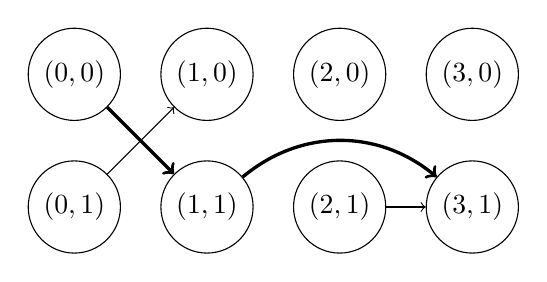
\begin{tikzpicture}[->,auto,node distance=0.5cm]
       \node[state] (q_0)                      {$(0, 0)$};
       \node[state] (q_1) [right=of q_0] {$(1, 0)$};
       \node[state] (q_2)  [right=of q_1] {$(2, 0)$};
       \node[state] (q_3) [right=of q_2] {$(3, 0)$};
       \node[state] (q_4)  [below=of q_0] {$(0, 1)$};
       \node[state] (q_5)  [right=of q_4] {$(1, 1)$};
      \node[state] (q_6)  [right=of q_5] {$(2, 1)$};
       \node[state] (q_7)  [right=of q_6] {$(3, 1)$};
       \path[->]
        (q_0) edge[very thick]  node {} (q_5)
        (q_4) edge  node {} (q_1)
        (q_5) edge [bend left, out=40, in=140, below, very thick]  node {} (q_7)
        (q_6) edge   node {} (q_7)
        ;
    \end{tikzpicture}
    \caption{The Kronecker product graph of RSM $R$ and the input graph $\mathcal{G}$ (edges which form new paths are thick)}
    \label{fig:example_1_product}
\end{figure}

This path starts in the vertex $(0,0)$ and finishes in the vertex $(3,1)$.
We can see, that 0 and 3 are the start and final states of some component
state machine for label $S$ in $R$ respectively. Thus we can conclude that
there exists a path between vertices 0 and 1 in the graph, such that the
respective word is derivable from $S$ in the $R$ execution flow.

As a result, we can add the edge $(0,S,1)$ to the resulting graph, what is done by updating the matrix $M_2^S$.

\textbf{The second iteration.} The modified graph Boolean adjacency matrices contain
an edge with label $S$. Therefore, this label contributes to the non-empty
corresponding matrix block in the evaluated matrix $M_{3,{2}}$. The transitive closure
evaluation introduces three new paths $(0, 1) \rightarrow (2,1), (1, 0) \rightarrow (3,1)$ and $(0, 1) \rightarrow (3,1)$ (see Figure~\ref{fig:example_2_product}). Since only the path between vertices $(0,1)$ and
$(3,1)$ connects the start and final states in the automaton, the edge $(1,S,1)$ is added to the resulting graph.
{
    \renewcommand{\arraystretch}{0.5}
    \setlength\arraycolsep{0.1pt}
\begin{align*}
  \centering
& M_{3,(2)} = M_1^a \otimes M_{2,(2)}^a +  M_1^b \otimes M_{2,(2)}^b + M_1^S \otimes M_{2,(2)}^S = \\
& \kbordermatrix{
          & (0,0) & (0,1) & \vrule & (1,0) & (1,1) & \vrule &  (2,0) & (2,1) & \vrule &  (3,0) & (3,1) &\\
    (0,0) & . & .  & \vrule & . & 1  & \vrule & . & .  &  \vrule & . & .  \\
    (0,1) & . & .  & \vrule & 1 & .   & \vrule & . & .  &  \vrule & . & .  \\
    \hline
    (1,0) & . & .   & \vrule & . & .  & \vrule & . & \mc  & \vrule & . & . \\
    (1,1) & . & .   & \vrule & . & .  & \vrule & . & .  & \vrule & .  &1   \\
    \hline
    (2,0) & . & .   & \vrule & . & .  & \vrule & . & .  & \vrule & . & .  \\
    (2,1) & . & .   & \vrule & . & .  & \vrule & . & .  & \vrule & . &1  \\
    \hline
    (3,0) & . & .   & \vrule & . & .  & \vrule & . & .  & \vrule & . & .  \\
    (3,1) & . & .   & \vrule & . & .  & \vrule & . & .  & \vrule & . & .  \\
}
\end{align*}
}
\begin{figure}[h]
    \centering
   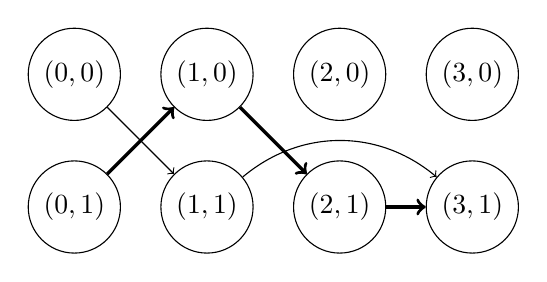
\begin{tikzpicture}[->,auto,node distance=0.5cm]
       \node[state] (q_0)                      {$(0, 0)$};
       \node[state] (q_1) [right=of q_0] {$(1, 0)$};
       \node[state] (q_2)  [right=of q_1] {$(2, 0)$};
       \node[state] (q_3) [right=of q_2] {$(3, 0)$};
       \node[state] (q_4)  [below=of q_0] {$(0, 1)$};
       \node[state] (q_5)  [right=of q_4] {$(1, 1)$};
      \node[state] (q_6)  [right=of q_5] {$(2, 1)$};
       \node[state] (q_7)  [right=of q_6] {$(3, 1)$};
       \path[->]
        (q_1) edge[very thick] node {} (q_6)
        (q_0) edge node {} (q_5)
        (q_4) edge[very thick]  node {} (q_1)
        (q_5) edge [bend left, in=140, out=40, below]  node {} (q_7)
        (q_6) edge[very thick]   node {} (q_7)
        ;
    \end{tikzpicture}
    \caption{The Kronecker product graph of RSM $R$ and the updated graph $\mathcal{G}$ (edges which form new paths are thick)}
    \label{fig:example_2_product}
\end{figure}
The result graph is presented in Figure~\ref{fig:example_result}.
\begin{figure}[h]
    \centering
    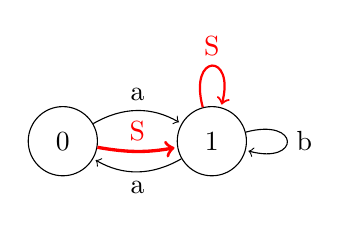
\begin{tikzpicture}[shorten >=1pt,auto]
       \node[state] (q_0)                      {$0$};
       \node[state] (q_1) [right=of q_0]       {$1$};
        \path[->]
        (q_0) edge[bend left, above]   node {a} (q_1)
         (q_0) edge[in=190, out=-10, red, very thick]   node {S} (q_1)
        (q_1) edge [bend left, below] node {a} (q_0)
         (q_1) edge[loop above, red, thick] node {S} (q_1)
        (q_1) edge[loop right] node {b} (q_1);

    \end{tikzpicture}
    \caption{The result graph $\mathcal{G}$}
    \label{fig:example_result}
\end{figure}


\begin{figure}[h]
	\centering
	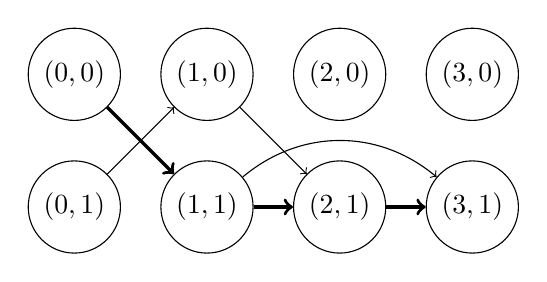
\begin{tikzpicture}[->,auto,node distance=0.5cm]
		\node[state] (q_0)                      {$(0, 0)$};
		\node[state] (q_1) [right=of q_0] {$(1, 0)$};
		\node[state] (q_2)  [right=of q_1] {$(2, 0)$};
		\node[state] (q_3) [right=of q_2] {$(3, 0)$};
		\node[state] (q_4)  [below=of q_0] {$(0, 1)$};
		\node[state] (q_5)  [right=of q_4] {$(1, 1)$};
		\node[state] (q_6)  [right=of q_5] {$(2, 1)$};
		\node[state] (q_7)  [right=of q_6] {$(3, 1)$};
		\path[->]
		(q_1) edge node {} (q_6)
		(q_0) edge[very thick] node {} (q_5)
		(q_4) edge  node {} (q_1)
		(q_5) edge [bend left, in=140, out=40, below]  node {} (q_7)
		(q_5) edge[very thick]   node {} (q_6)
		(q_6) edge[very thick]   node {} (q_7)
		;
	\end{tikzpicture}
	\caption{The Kronecker product graph of RSM $R$ and the final graph $\mathcal{G}$ (edges which form new paths are thick)}
	\label{fig:example_3_product}
\end{figure}


No more edges will be added to the graph $\mathcal{G}$ at the last iteration.
However, the new edge $(1, 1) \rightarrow (2,1)$ will be added to the resulting Kronecker product, and the transitive closure
evaluation introduces one new path $(0, 0) \rightarrow (3,1)$ that connects the start and final states in the automaton (see Figure~\ref{fig:example_3_product}).
At this point, the index creation is finished.
One can use it to answer reachability queries, but it also can be used
to restore paths for some reachable vertices. The resulting Kronecker product matrix
$M_3$, or so-called \textit{index}, can be used for it.
For example, we can restore paths from vertex 1 to vertex 1 derived from $S$ in the resulting graph.

To get these paths we should call \verb|getPaths(1, 1, S)| function.
A partial trace of this call is presented in Figure~\ref{trc:example}.
First, we query paths for all possible start and final states of the
machine for the provided graph vertices.
Since the component state machine with label $S$ in the example RSM has the single final state, the function \verb|genPaths| is called with the arguments $(0,1)$ and $(3,1)$.
Note, that the values passed to the functions in the path extraction algorithm are the
pairs of the machine state and graph vertex, which uniquely identify a cell of
the index matrix $M_3$. As a result,
we get the set of all possible paths in the graph from $1$ to $1$ derived from $S$.

\begin{figure}
\begin{minipage}[t]{0.48\textwidth}
{
\scriptsize
\setlength{\DTbaselineskip}{8pt}
\DTsetlength{0.2em}{0.5em}{0.2em}{0.4pt}{1.6pt}
\dirtree{%
.1 getPaths($1,1,S$).
.2 genPaths($(0,1),(3,1)$).
.3 return $\{[((0,1),(1,0)), ((1,0),(2,1)), ((2,1),(3,1))]\}$.
.2 currentSubPaths = $\{[1 \xrightarrow{a} 0]\}$.
.2 currentPaths = $\{[(1 \xrightarrow{a} 0)]\}$.
.2 getPaths($0,1,S$).
.3 genPaths($(0,0),(3,1)$).
.4 return $\{[((0,0),(1,1)), ((1,1),(3,1))], [((0,0),(1,1)), ((1,1),(2,1)), ((2,1),(3,1))]\}$.
.3 path = $[((0,0),(1,1)), ((1,1),(3,1))]$.
.3 currentSubPaths = $\{[0 \xrightarrow{a} 1]\}$.
.3 currentPaths = $\{[0 \xrightarrow{a} 1]\}$.
.3 currentSubPaths = $\{[1 \xrightarrow{b} 1]\}$.
.3 $\cdots$.
.3 resultPaths = $\{[0 \xrightarrow{a} 1 \xrightarrow{b} 1]\}$.
.3 path = $[((0,0),(1,1)), ((1,1),(2,1)), ((2,1),(3,1))]$.
.3 currentSubPaths = $\{[0 \xrightarrow{a} 1]\}$.
.3 currentPaths = $\{[0 \xrightarrow{a} 1]\}$.
.3 getPaths(1, 1, S) // \begin{minipage}[t]{14cm} An alternative way to get paths from 1 to 1 (leads to infinite set of paths) \end{minipage}.
.3 $\cdots$.
.8 return $r_\infty^{1 \leadsto 1}$ // \begin{minipage}[t]{5cm} An infinite set of path from 1 to 1 \end{minipage}.
.3 currentPaths = $\{[0 \xrightarrow{a} 1] \} \cdot r_\infty^{1\leadsto 1}$.
.3 currentSubPaths = $\{[1 \xrightarrow{b} 1]\}$.
.3 $\cdots$.
.3 return $\{[0 \xrightarrow{a} 1 \xrightarrow{b} 1]\} \cup (\{[0 \xrightarrow{a} 1] \} \cdot r_\infty^{1\leadsto 1} \cdot \{[1 \xrightarrow{b} 1]\})$.
.2 currentPaths = $\{[1 \xrightarrow{a} 0 \xrightarrow{a} 1 \xrightarrow{b} 1]\} \cup (\{[1 \xrightarrow{a} 0 \xrightarrow{a} 1] \} \cdot r_\infty^{1\leadsto 1} \cdot \{[1 \xrightarrow{b} 1]\})$.
.2 currentSubPaths = $\{[1 \xrightarrow{b} 1]\}$.
.2 $\cdots$.
.2 return = $\{[1 \xrightarrow{a} 0 \xrightarrow{a} 1 \xrightarrow{b} 1 \xrightarrow{b} 1]\} \cup (\{[1 \xrightarrow{a} 0 \xrightarrow{a} 1] \} \cdot r_\infty^{1\leadsto 1} \cdot \{[1 \xrightarrow{b} 1 \xrightarrow{b} 1]\})$.
}
}
\caption{Example of call stack trace}
\label{trc:example}
\end{minipage}
\end{figure}
\section{Evaluation}

For performance analysis of proposed solution we evaluated some most common graph algorithms using real-world sparse matrix data. 
As a baseline for comparison we chose LAGraph~\cite{szarnyas2021lagraph} in connection with SuiteSparse~\cite{10.1145/3322125} as a CPU tool, Gunrock~\cite{7967137} and GraphBLAST~\cite{yang2019graphblast} as a Nvidia GPU tools. 
Also, we tested algorithms on several devices with distinct OpenCL vendors in order to validate portability of the proposed solution. 
In general, these evaluation intentions are summarized in the following research questions. 

\vspace{0.2cm}
\begin{itemize}
    \item[\textbf{RQ1}] What is the performance of the proposed solution relative to existing tools for both CPU and GPU analysis?
    
    \item[\textbf{RQ2}] What is the portability of the proposed solution with respect to various device vendors and OpenCL runtimes?
\end{itemize}

\subsection{Evaluation Setup}

For evaluation, we use a PC with Ubuntu 20.04 installed, which has 3.40Hz Intel Core i7-6700 4-core CPU, DDR4 64Gb RAM, and Nvidia GeForce GTX 1070 GPU with 8Gb VRAM. 
Host programs were compiled with GCC 9.3.0 compiler. Programs using CUDA were compiled with GCC 8.4.0 and Nvidia NVCC 10.1.243 compiler.
Release mode and maximum optimization level was enabled for all tested programs. 
Data loading time, preparation, format transformations and host-device initial communications are excluded from time measurements. 
All tests are averaged across 10 runs.
Additional warm-up run for each test execution is excluded from measurements.

\subsection{Graph Algorithms}

For preliminary study \textit{breadth-first search} (bfs) and \textit{triangles counting} (tc) algorithms were chosen, since they allows analyse the performance of \textit{vxm} and \textit{mxm} operations, rely heavily on \textit{masking}, and utilize \textit{reduction} or \textit{assignment}. 
BFS implementation utilizes automated vector storage from sparse to dense switch and only \textit{}{push optimization}. 
TC implementation uses masked \textit{mxm} of source lower-triangular matrix with second transposed argument.

\subsection{Dataset}

Nine graph matrices were selected from the Sparse Matrix Collection at University of Florida~\cite{dataset:10.1145/2049662.2049663}. 
Information about graphs is summarized in Table~\ref{dataset:info}. 
All datasets are converted to undirected graphs. 
Self-loops and duplicated edges are removed.

\begin{table}[htbp]
\caption{Dataset description.} 
\begin{center}
    \rowcolors{2}{black!2}{black!10}
    \begin{tabular}{|l|r|r|r|}
    \hline
    Dataset & Vertices  & Edges & Max Degree \\
    \hline
    \hline
    coAuthorsCiteseer & 227.3K &   1.6M &    1372 \\
    coPapersDBLP      & 540.4K &  30.4M &    3299 \\
    hollywood-2009    &   1.1M & 113.8M &  11,467 \\
    roadNet-CA        &   1.9M &   5.5M &      12 \\
    com-Orkut         &     3M &   234M &   33313 \\
    cit-Patents       &   3.7M &  16.5M &     793 \\
    rgg\_n\_2\_22\_s0 &   4.1M &  60.7M &      36 \\
    soc-LiveJournal   &   4.8M &  68.9M &  20,333 \\
    indochina-2004    &   7.5M & 194.1M & 256,425 \\
    \hline
    \end{tabular}
    \label{dataset:info}
\end{center}
\end{table}

\subsection{Results}

Table~\ref{results} presents results of the evaluation and compares performance of Spla against other tool on different execution platforms.
Tools are grouped by the type of the device for the execution, where either Nvidia GPU or Intel CPU are used. 
Cell left empty if tested tool failed to analyse graph due to \textit{out of memory} exception.

In general, Spla BFS shows acceptable performance, especially on graphs with large vertex degree, such as soc-LiveJournal and com-Orkut.
On graphs roadNet-CA and rgg it has a significant performance drop due to the nature of underlying algorithms and data structures. 
Firstly, library utilizes immutable data buffers. Thus, iteratively updated dense vector of reached vertices must be copied for each modification, what dominates the performance of the library on a graph with large search depth. 
Secondly, Spla BFS does not utilise \textit{pull optimization}, what is critical in a graph with relatively small search frontier. 

Spla TC has a good performance on GPU, which is better in all cases that reference SuiteSparse solution. 
But in most tests GPU competitors, especially Gunrock, show smaller processing times. 
GraphBLAST shows better performance as well. 
Library utilises masked SpGEMM algorithm, the same as in GraphBLAST, but without \textit{identity} element to fill gaps. 
Library explicitly stores all non-zero elements, and uses mask to reduce only non-zero while evaluating dot products of rows and columns. 
What causes extra divergence inside work groups. 
On Intel device Spla shows better performance compared to SuiteSparse on com-Orkut, cit-Patents and soc-LiveJournal. 
A possible reason is the large lengths of processed rows and columns in the product of matrices.

Gunrock shows nearly best average performance due to its specialized and optimized algorithms.
Also, it has good time characteristics on a mentioned earlier roadNet-CA and rgg in BFS algortihm. 
GraphBLAST follows Gunrock and show good performance as well. 
But it runs out of memory on a two significantly large graphs con-Orkut and indochina-2004. 
Spla does not rut out of memory on any test due to simplified storage scheme.

\begin{table}[htbp]
\caption{Graph algorithms evaluation results.\\Time in milliseconds (lower is better).} 
\begin{center}
    \begin{tabular}{|l|r|r|r|r|r|}
    \hline
    \multirow{2}{*}{Dataset} & \multicolumn{3}{c|}{Nvidia} & \multicolumn{2}{c|}{Intel} \\
    \cline{2-6}
    & GR & GB & SP & SS & SP \\
    \hline
    \hline
    \multicolumn{6}{|c|}{BFS} \\
    \hline
    \rowcolor{black!10} hollywood-2009    &  20.3 &  82.3 &   36.9 &   23.7 &   303.4 \\
    \rowcolor{black!2 } roadNet-CA        &  33.4 & 130.8 & 1456.4 &  168.2 &   965.6 \\
    \rowcolor{black!10} soc-LiveJournal   &  60.9 &  80.6 &   90.6 &   75.2 &  1206.3 \\
    \rowcolor{black!2 } rgg\_n\_2\_22\_s0 &  98.7 & 414.9 & 4504.3 & 1215.7 & 15630.1 \\
    \rowcolor{black!10} com-Orkut         & 205.2 & -- -- &  117.9 &   43.2 &   903.6 \\
    \rowcolor{black!2 } indochina-2004    &  32.7 & -- -- &  199.6 &  227.1 &  2704.6 \\
    \hline
    \hline
    \multicolumn{6}{|c|}{TC} \\
    \hline
    \rowcolor{black!10} coAuthorsCiteseer &   2.1 &    2.0 &    9.5 &    17.5 &    64.9 \\
    \rowcolor{black!2 } coPapersDBLP      &   5.7 &   94.4 &  201.9 &   543.1 &  1537.8 \\
    \rowcolor{black!10} roadNet-CA        &  34.3 &    5.8 &   16.1 &    47.1 &   357.6 \\
    \rowcolor{black!2 } com-Orkut         & 218.1 & 1583.8 & 2407.4 & 23731.4 & 15049.5 \\
    \rowcolor{black!10} cit-Patents       &  49.7 &   52.9 &   90.6 &   698.3 &   684.1 \\
    \rowcolor{black!2 } soc-LiveJournal   &  69.1 &  449.6 &  673.9 &  4002.6 &  3823.9 \\
    \hline
    \hline
    \multicolumn{6}{l}{Tools: Gunrock (GR), GraphBLAST (GB), SuiteSparse (SS), Spla (SP).} \\
    \end{tabular}
    \label{results}
\end{center}
\end{table}
 
% Two GPU

% \begin{table}[htbp]
%     \caption{Table Type Styles}
%     \begin{center}
%     \begin{tabular}{|c|c|c|c|}
%     \hline
%     \textbf{Table}&\multicolumn{3}{|c|}{\textbf{Table Column Head}} \\
%     \cline{2-4} 
%     \textbf{Head} & \textbf{\textit{Table column subhead}}& \textbf{\textit{Subhead}}& \textbf{\textit{Subhead}} \\
%     \hline
%     copy& More table copy$^{\mathrm{a}}$& &  \\
%     \hline
%     \multicolumn{4}{l}{$^{\mathrm{a}}$Sample of a Table footnote.}
%     \end{tabular}
%     \label{tab2}
%     \end{center}
% \end{table}

\section{Related work}
\label{sec:related}
\subsection{CFL-reachability}
The CFL-reachability problem was introduced by Yannakakis~\cite{Yannakakis} to describe the Datalog chain query evaluation problem. Later, Reps et al.~\cite{10.1145/222124.222146, 10.5555/271338.271343, SAGIV1996131} proposed the CFL-reachability framework for interprocedural program analysis. Since then the CFL-reachability has been used to formulate a variety of static analyses, such as points-to and alias analysis~\cite{ 10.1145/3158118, 10.1145/2814270.2814307,  10.1145/3450492, 10.1145/3360574, 10.1007/978-3-642-37051-9_4, 10.1145/2351676.2351720, 10.1145/1103845.1094817, 10.1145/2491956.2462159, 10.1145/2660193.2660213, Zheng:2008:DAA:1328897.1328464}, data-dependence analysis~\cite{10.1145/3158118}, type inference analysis~\cite{10.1145/2647508.2647522}, type-base flow analysis~\cite{10.1145/360204.360208} and program slicing~\cite{10.1145/193173.195287}.

A cubic $O(n^3)$ algorithm for the CFL-reachability which uses dynamic programming technique, was proposed by Melski and Reps~\cite{10.1145/258994.259006}. This result was improved by a logarithmic factor by Chaudhuri~\cite{Chaudhuri2008SubcubicAF}, giving the worst-case runtime complexity $O(n^3/\log n)$. Unfortunately, no algorithm faster has been discovered, for general graphs with $n$ vertices and general context-free grammars, so the CFL-reachability is known to have a ``cubic bottleneck''~\cite{10.5555/788019.788876}. Recent result by Chatterjee et al.~\cite{10.1145/3158118} shows that the CFL-reachability in cubic time is optimal under combinatorial Boolean Matrix Multiplication (BMM) hypothesis. The cubic lower bound under the same hypothesis was also established for Andersen's Pointer Analysis directly~\cite{pavlogiannis2020finegrained}. The cubic runtime can be improved substantially in specific cases, by taking advantage of certain properties of the underlying graph (i.e. bidirected graphs)~\cite{10.1145/3158118, 10.1145/2491956.2462159} or grammar/context-free language (i.e. Dyck language of 1 parenthesis)~\cite{8249039, pavlogiannis2020finegrained}.

There are some algorithms in the context of database theory, where exists the equivalent problem called Context-Free Path Querying (CFPQ)~\cite{Azimov:2018:CPQ:3210259.3210264, Grigorev:2017:CPQ:3166094.3166104, hellingsPathQuerying, Medeiros:2018:EEC:3167132.3167265, 10.1007/978-3-030-54832-2_6, 10.1007/978-3-319-91662-0_17, 10.1145/3398682.3399163, 10.1007/978-3-319-41579-6_22}. It is important to mention that some of these algorithms reduce CFPQ evaluation to linear algebra operations: Azimov et al.~\cite{Azimov:2018:CPQ:3210259.3210264} reduce CFPQ to matrix multiplication and Orachev et al.~\cite{10.1007/978-3-030-54832-2_6} reduce CFPQ to Kronecker product. Additionally, recently Sato~\cite{sato_2017} proposed linear algebraic approach to Datalog evaluation. This approach is based on the transformation of Datalog program to a set of matrix equations, and can be used for Datalog chain queries evaluation which is equivalent to the CFL-reachability problem. Unfortunately, all three mentioned algorithms have worse than cubic $O(n^5)$ theoretical time complexity, whereas our algorithm has state-of-the-art theoretical time complexity, having all the advantages of linear algebra formulation at the same time.

\subsection{Graph processing systems}

State-of-the-art systems for large graph proccessing use different architectures including single‑machine and shared‑memory parallel ones~\cite{10.1145/3064176.3064191, 10.1145/2723372.2735369, 10.1145/2442516.2442530, Wang2013AsynchronousLG, 10.1145/2688500.2688507}, multi-core and multi-processor architectures \cite{10.1177/1094342011403516, Gregor2005ThePB, 6569865}, and distributed graph processing systems~\cite{ 10.1145/3087556.3087580, 10.1145/2621934.2621936, Jia2017ADM, Khorasani2014CuShaVG, 10.14778/2212351.2212354, 10.1145/2517349.2522740, Sengupta2016GraphInAO, 10.1145/3016078.2851145, Yan2018GraphDDV, 10.5555/1863103.1863113}. However, it is hard to use these engines for the implementation of the interprocedural program analysis tool without ground-up redesign~\cite{10.1145/3037697.3037744}.

There are many works which formulate specific graph algorithms in terms of linear algebra, for example, such algorithms as for computing transitive closure and all-pairs shortest paths.
Recently this direction was summarized in GraphBLAS API~\cite{7761646} which provides building blocks to develop a graph analysis algorithm in terms of linear algebra.
There is a number of implementations of this API, such as SuiteSparse:GraphBLAS~\cite{10.1145/3322125}, CombBLAS~\cite{10.1177/1094342011403516}, GraphBLAST~\cite{yang2019graphblast}, GraphMat~\cite{10.14778/2809974.2809983}, GraphPad~\cite{7516027}. 

We implemented our tool on top of SuiteSparse:GraphBLAS because it gives a very flexible and convenient way to construct graph algorithms by using primitive and highly-optimized building blocks based on the set of of sparse matrix operations.
\subsection{CFL-reachability-based code analysis tools}
Since CFL-reachability captures a certain sub-class of Datalog, Datalog can be employed as a domain specific language to express custom program analyses, reducing the complexity of developing program analyzers. Such Datalog-powered tools, which are able to run sophisticated static analysis include bddbddb~\cite{10.1007/11575467_8}, DOOP~\cite{10.1145/1640089.1640108}, LogicBlox~\cite{10.1145/2723372.2742796}, $\mu$Z~\cite{10.1007/978-3-642-22110-1_36}, Souffl{\'e}~\cite{10.1007/978-3-319-41540-6_23}. However, such engines are known to be fundamentally limited by the size of main memory and, therefore, are not able to scale well on a large code systems~\cite{10.1145/3453483.3454085}, and experience reduced performance compared to manually implemented tools~\cite{10.1007/978-3-319-41540-6_23}.

A single-machine, disk-based graph systems Grapple~\cite{10.1145/3302424.3303972}, Graspan~\cite{10.1145/3037697.3037744} and Chianina~\cite{10.1145/3453483.3454085} turn code analysis into bigdata analytics. The main goal of Graspan is to scale context-free CFL-reachability based analyses to large programs with disk support. A piece of work Chianina~\cite{10.1145/3453483.3454085} supports easy development of any context- and flow-sensitive analysis for C. Unfortunately, massive expensive disk I/Os remain the major performance bottleneck of disk-based graph processing.


\section{Conclusion}

In this paper we present a library for sparse Boolean linear algebra which implements such basic operations as matrix-matrix multiplication and element-wise matrix-matrix addition in both Cuda and OpenCL.
Evaluation shows that our Boolean-specific implementations faster and require less memory than generic, not the Boolean optimized, operations from state-of-the-art libraries. 
Thus, the specialization of operations for this data type makes sense. 

The first direction of the future work is to integrate all parts (OpenCL and Cuda backends) into a single library and improve its documentation and prepare to publish.
Moreover, it is necessary to extend the library with other operations, including matrix-vector operations, masking, and so on.
As a result a Python package should be published.

Another important step is to evaluate the library on different algorithms and devices.
Namely, algorithms for RPQ and CFPQ should be implemented and evaluated on related data sets.
Also, it is necessary to evaluate OpenCL version on FPGA which may require additional technical effort and code changes.

Finally, we plan to discuss with GraphBLAS community possible ways to use our library as a backend for GraphBLAST or SuiteSparse in case of Boolean computations.
Moreover, it may be possible to use implemented algorithms as a foundation for generalization to arbitrary semirings.



%% Acknowledgments
\begin{acks}                            %% acks environment is optional
                                        %% contents suppressed with 'anonymous'
  %% Commands \grantsponsor{<sponsorID>}{<name>}{<url>} and
  %% \grantnum[<url>]{<sponsorID>}{<number>} should be used to
  %% acknowledge financial support and will be used by metadata
  %% extraction tools.
 The research was supported by the Russian Science Foundation, grant number: 18-11-00100. Any opinions, findings, and
  conclusions or recommendations expressed in this material are those
  of the author and do not necessarily reflect the views of the
  National Science Foundation.
\end{acks}


%% Bibliography
%\bibliography{bibfile}
\bibliography{tensor_product_CFL-reach}


%% Appendix
\appendix
\section{Appendix}

Text of appendix \ldots

\end{document}
